%% LyX 2.2.3 created this file.  For more info, see http://www.lyx.org/.
%% Do not edit unless you really know what you are doing.
\documentclass[oneside,english,titlepage]{amsart}
\usepackage{lmodern}
\usepackage{lmodern}
\usepackage[T1]{fontenc}
\usepackage{geometry}
\geometry{verbose,tmargin=1in,bmargin=1in,lmargin=1in,rmargin=1in}
\usepackage{babel}
\usepackage{float}
\usepackage{mathtools}
\usepackage{amstext}
\usepackage{amsthm}
\usepackage{stmaryrd}
\usepackage{graphicx}
\usepackage{setspace}
\doublespacing
\usepackage[unicode=true,
 bookmarks=false,
 breaklinks=false,pdfborder={0 0 1},backref=section,colorlinks=false]
 {hyperref}

\makeatletter
%%%%%%%%%%%%%%%%%%%%%%%%%%%%%% Textclass specific LaTeX commands.
\numberwithin{equation}{section}
\numberwithin{figure}{section}

%%%%%%%%%%%%%%%%%%%%%%%%%%%%%% User specified LaTeX commands.
\usepackage{flafter}




\usepackage{babel}

\@ifundefined{showcaptionsetup}{}{%
 \PassOptionsToPackage{caption=false}{subfig}}
\usepackage{subfig}
\makeatother

\begin{document}
\begin{singlespace}
\noindent \pagenumbering{gobble}
\end{singlespace}
\begin{singlespace}

\title{\noindent Graphical LASSO and its Applications}
\end{singlespace}
\begin{singlespace}

\author{\noindent Alex Wasielewski, Hengrui Luo, Nate Wilairat, Xiaofei Zhou}
\end{singlespace}
\begin{abstract}
\begin{singlespace}
\noindent In this report we discuss the theoretic motivation for the
graphical LASSO methodology and conducted corresponding simulation
studies on simulated and real datasets. A thorough discussion of two
approaches toward the derivation of graphical LASSO are covered in
the first part of the paper. In the second part of the paper a careful
data analysis is carried out with appropriate comparison and tuning
of parameters. We ended up with the report with a discussion about
the graphical LASSO as well as its features. 
\end{singlespace}
\end{abstract}

\maketitle
\begin{singlespace}
\noindent \tableofcontents{}

\noindent \newpage{}\pagenumbering{arabic}
\end{singlespace}
\begin{singlespace}

\section{Introduction to Graphical Models}
\end{singlespace}
\begin{singlespace}

\subsection{Gaussian Graphical model and its applications}
\end{singlespace}

\begin{singlespace}
\noindent Graphical models are used everywhere with applications in
imaging, network analysis, and Bayesian statistics. It is always of
central interest to investigate the dependency relations in the graph
model. In this report we briefly introduce the formulation of the
problem of estimating the covariance matrix when the underlying probabilistic
model of an undirected graph is assumed to be Gaussian. And following
\cite{FHT2008,FHT2001,Meinshausen=00003D000026B=00003D0000FChlmann2006},
we explain how the covariance estimation problem for Gaussian process
can be regarded as a regression problem as well as a neighborhood
detection problem for the undirected graph. Once we establish these
perspectives, we can apply classic regression techniques like LASSO
when the dimension of the random variables in the undirected graph
is high, even for $p>n$. Traditionally this presents difficulty in
estimation as well as consistency of the estimators, however a penalized
likelihood estimate like LASSO can accommodate the problem neatly
with high efficiency.

\noindent The model for continuous i.i.d. $p$-dimensional data $X=(X_{1},\cdots,X_{p})$
assumes that the random variables are represented by vertices in the
graph and distributed as a multivariate Gaussian distribution $N_{p}(\mu,\Sigma)$
with mean $\text{\ensuremath{\mu}}$ and covariance matrix $\Sigma$,
or equivalently the precision matrix $\Theta=\Sigma^{-1}$, respectively.
In an undirected graph, the random variables are represented by the
vertices and the conditional dependency relations are represented
by edges connecting two vertices. If there is no edge between two
vertices, then it means that the corresponding pair of random variables
associated with the vertices are conditionally independent given all
the rest of the random variables represented by all other vertices
in the graph. Let us consider the following example from \cite{FHT2001}.
This kind of rule actually provides a way of representing the dependency
structure between Gaussian variables.

\noindent 
\begin{figure}[H]
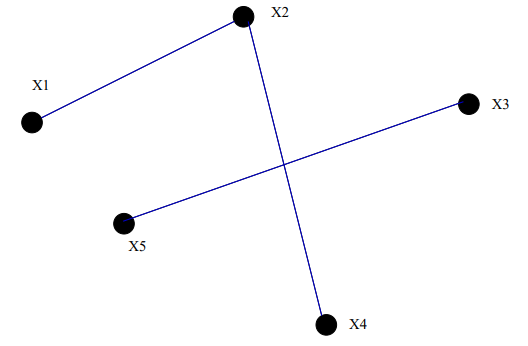
\includegraphics[scale=0.5]{pasted1} \caption{\label{fig:Simple-example-of}Simple example of $\{X_{1},\cdots,X_{5}\}$
represented by an undirected graphs}
\end{figure}

\noindent In the Figure \ref{fig:Simple-example-of}, we used an example
from \cite{FHT2001}. We will refer to this example in the following
section.
\end{singlespace}
\begin{singlespace}

\subsection{Representation of undirected graphs}
\end{singlespace}

\begin{singlespace}
\noindent Consider the adjoint matrix (or adjacent matrix or edge
matrix) representation of this graph Figure \ref{fig:Simple-example-of},
we get a $5\times5$ matrix where 1 means two vertices are joined
and 0 means they are not joined. Then the adjoint matrix can be viewed
as a forgetful image of the inverse covariance matrix. If we replace
the entries in the adjoint matrix with the covariance between two
vertices, then we can transform the adjoint matrix into the covariance
matrix. Similarly we can also consider their correlation matrix after
normalization by their respective variances. 
\begin{align*}
\left(\begin{array}{ccccc}
1 & 1 & 0 & 0 & 0\\
1 & 1 & 0 & 1 & 0\\
0 & 0 & 1 & 0 & 1\\
0 & 1 & 0 & 1 & 0\\
0 & 0 & 1 & 0 & 1
\end{array}\right) & \leftrightarrow\left(\begin{array}{ccccc}
Cov(X_{1},X_{1}) & Cov(X_{2},X_{1}) & 0 & 0 & 0\\
Cov(X_{1},X_{2}) & Cov(X_{2},X_{2}) & 0 & Cov(X_{4},X_{2}) & 0\\
0 & 0 & Cov(X_{3},X_{3}) & 0 & Cov(X_{5},X_{3})\\
0 & Cov(X_{2},X_{4}) & 0 & Cov(X_{4},X_{4}) & 0\\
0 & 0 & Cov(X_{3},X_{5}) & 0 & Cov(X_{5},X_{5})
\end{array}\right)
\end{align*}

\noindent For the Gaussian multivariate distribution, the precision
matrix captures the conditional distribution of each $X_{j},j=1,\cdots,p$.
To see this point we consider the case $p=2$, 
\begin{align*}
N_{2}(\mu,\Sigma) & =N_{2}\left(\left(\begin{array}{c}
\mu_{1}\\
\mu_{2}
\end{array}\right),\left(\begin{array}{cc}
\sigma_{11} & \sigma_{12}\\
\sigma_{21} & \sigma_{22}
\end{array}\right)\right)
\end{align*}
and $X_{1}\mid X_{2}=a\sim N\left(\mu_{1}+\sigma_{12}\sigma_{22}^{-2}(a-\mu_{2}),\sigma_{11}-\sigma_{12}\sigma_{22}^{-1}\sigma_{21}\right)$.
The precision matrix of $\Sigma$ is 
\begin{align*}
\Theta & =\left(\begin{array}{cc}
\sigma_{22} & -\sigma_{12}\\
-\sigma_{21} & \sigma_{11}
\end{array}\right)\cdot\frac{1}{\sigma_{11}\sigma_{22}-\sigma_{12}\sigma_{21}}
\end{align*}
and we can regard the edges in a undirected graph as the nonzero entries
in the precision matrix and the zero entries means conditional independence
between two variables. The reason why we use the precision matrix
instead of covariance matrix directly is that we are capturing the
conditional dependency between $X$'s, whose distribution is parameterized
by the precision matrix. In another sense, the conditional expectation,
as the best linear unbiased predictor (BLUP) and $L^{2}$ optimizer,
also makes use of the precision matrix in a closed form expression
and thus can capture the conditional dependence better. We will also
see later that this is a natural choice in terms of algorithmic consideration.

\noindent Take the covariance matrix as a functional of the data generating
mechanism. The estimation of this functional can be reduced to discrete
optimization problem. However, the computational complexity for an
exhaustive method of estimation of the covariance matrix is generally
exponential \cite{FHT2008,FHT2001} and therefore not appropriate.
Also, we want to take into consideration the dependence structure
exhibited in the undirected graph when making inference, especially
when the data is sparse. These two concerns jointly lead to the invention
of graphical LASSO, a mixture of two methods which can take care of
the sparsity and efficient computing problems.
\end{singlespace}
\begin{singlespace}

\section{Graphical LASSO and Neighborhood Detection}
\end{singlespace}

\begin{singlespace}
\noindent In the seminal paper \cite{Meinshausen=00003D000026B=00003D0000FChlmann2006},
the central problem is to estimate the covariance matrix. The author
proposed to estimate the pattern zeros in the covariance matrix, which
contains information about the conditional independence information
in the graph representation of the collection of observed random variables
$X=(X_{1},\cdots,X_{p})$. To estimate those structural zeros in the
covariance matrix is equivalent to estimating the neighborhood of
each vertex, through this perspective. The covariance estimation problem
can be regarded as discovering the conditional independence structure
contained in those i.i.d. observations. A stronger dependency between
two random variable vertices means a partial correlation in the correlation
matrix with absolute value closer to one; a weaker dependency between
two random variable vertices means a partial correlation in the correlation
matrix with absolute value closer to zero. Now we examine the conditional
distribution of $X_{j}\mid X_{-j}$ which means we conditioned on
all other vertices in the graph except for $X_{j}$. Since we assume
the underlying model is Gaussian, we can use the closed form conditional
distribution. In the following notations, we assume $\Sigma=\left\llbracket \sigma_{ij}\right\rrbracket _{i,j}^{n},\Sigma^{-1}=\Theta=\left\llbracket \theta_{ij}\right\rrbracket _{i,j}^{n}$
and more precisely $\theta_{ij}=-\sigma_{ij\mid-ij}\det\Sigma_{-ij}\det\Sigma^{-1}$
where $\sigma_{ij\mid-ij}$ is the marginal covariance conditioning
on all other random variables except for the $i,j$-th random variables;
$\Sigma_{-ij}$ is the covariance matrix with the $i$-th row and
$j$-th column removed. We then have, 
\begin{align*}
X_{j}\mid X_{-j}\sim & N_{1}\left(\sum_{i\neq j}X_{i}\beta_{ij},\sigma_{jj}\right)\\
\beta_{ij} & =-\frac{\theta_{ij}}{\theta_{jj}}\\
\sigma_{jj} & =\frac{1}{\theta_{jj}}
\end{align*}
If we regarded the partial correlation between two random variables
as geometric ``angles'' between two random variables, the closed
form of the conditional distribution above shows that the mean of
$X_{j}\mid X_{-j}$ is the sum of projected images of $X_{j}$ onto
other random variables $X_{-j}=\left\{ X_{1},\cdots,X_{j-1},X_{j+1},\cdots,X_{n}\right\} $
and the variance is the norm of this mean. Moreover, 
\begin{align*}
\beta_{ij} & \propto\frac{\theta_{ij}}{\sqrt{\theta_{ii}\cdot\theta_{jj}}}
\end{align*}
and $\beta_{ij}=0\Leftrightarrow\theta_{ij}=0\Leftrightarrow X_{i}\perp X_{j}\mid X_{-ij}$
(i.e. $X_{i},X_{j}$ are independent conditioning on all other random
variables except for $i,j$-th random variable). For our example in
Figure 1.1, $X_{2}\perp X_{3}\mid X_{1},X_{4},X_{5}$. Therefore there
is an one-to-one correspondence between neighborhoods and nonzero
entries of the covariance matrix.

\noindent Observe that the conditional distribution with mean $\sum_{i\neq j}X_{i}\beta_{ij}$
of $X_{j}\mid X_{-j}$ can be regarded as a regression model. Therefore,
it is tempting to estimate the covariance matrix using the classic
estimate from the regression setup. That is to say we are trying to
estimate the response $X_{j}$ by regressing on the rest of the random
variables, $X_{-j}$, with coefficients $\beta_{ij},i\neq j$. Currently
based on the Gaussian graphical model, the author \cite{FHT2008}
proposed to derive the joint likelihood based (i.e. the joint likelihood
of $\left\{ X_{1},\cdots,X_{n}\right\} $) estimate 
\begin{align}
\ell_{\lambda}(\Theta) & =\log\det\Theta-Tr(S\Theta)\label{eq:logl}
\end{align}
such that $S$ is the empirical covariance matrix of the data. We
can differentiate with respect to the $\Theta$ and solve following
estimate equation 
\begin{align*}
\frac{\partial\ell(\Theta)}{\partial\Theta} & =\Theta^{-1}-S=0
\end{align*}
However, such an estimate is not very useful since it is simply the
moment estimate without considering the underlying dependence structure
provided by the undirected graph.

\noindent There are two ways of deriving the graphical LASSO method
from this point. One way is to follow \cite{Meinshausen=00003D000026B=00003D0000FChlmann2006},
that is to say we can regress each vertex $X_{j}$ as a regression
function of all the other random variables that is a neighbor to $X_{j}$
(i.e. there is at least an edge connecting $X_{j}$ and the vertex
representing the random variable). Again in our simplest example above,
$X_{2}$ is regressed on $X_{1},X_{4}$ only. Then $\widehat{\beta_{ij}}$
can be used for estimating the covariance/correlation between $X_{2}$
and other random variables respecting the structure of the undirected
graph. After doing the same regression procedure for each $X_{1},\cdots,X_{n}$
we can obtain an estimate for $\Sigma^{-1}$ and hence an estimate
to the covariance matrix with respect to the underlying graphical
dependency structure. If we take this approach, then this becomes
an obvious problem of iterative updating of each vertex in the undirected
graphs until the final solution to the estimate actually converges.
One common method that can be applied to fit this conditional model
is the cyclical coordinate descent algorithm \cite{Wright2015} that
optimizes the objective function (e.g. $L^{2}$ loss function) with
respect to only one regressor coordinate at one time and cyclically
updates coordinates until the algorithm converges.

\noindent The other way \cite{FHT2008} is to modify the likelihood
equation directly. Instead of doing a maximal likelihood equation,
we consider its $L^{1}$ penalized version of the likelihood above
with a tuning parameter $\lambda>0$. 
\begin{align}
\ell_{\lambda}(\Theta) & =\log\det\Theta-Tr(S\Theta)-\lambda\|\Theta\|_{1}\label{eq:plogl}
\end{align}
\begin{align*}
\frac{\partial\ell(\Theta)}{\partial\Theta} & =\Theta^{-1}-S-\lambda\cdot sgn\left(\Theta\right)=0
\end{align*}
where the function $sgn\left(\Theta\right)\coloneqq\left\llbracket sgn(\theta_{ij})\right\rrbracket _{ij}^{n}$
is simply applying the sign function to each entry of the precision
matrix. This reproduces our adjoint matrix representation of the undirected
graph. One step further we can realize that this is exactly the penalized
estimate equation of LASSO on regression coefficients. One comment
is that if we return to our geometric interpretation of the regression
coefficients $\beta_{ij}$ as ``angles'' between two random variables,
then the penalized estimation in this scenario is no more than scaling
the angles to achieve a dimension reduction for the space consisting
of the regression basis. Consider the following equation in $W$:
$W=\Theta^{-1}$.

\noindent 
\begin{align*}
\left(\begin{array}{cc}
W_{11} & w_{12}\\
w_{21} & w_{22}
\end{array}\right)_{p\times p}\left(\begin{array}{cc}
\Theta_{11} & \theta_{12}\\
\theta_{12}^{T} & \theta_{22}
\end{array}\right)_{p\times p} & =I_{p}
\end{align*}
by the partitioned matrix multiplication formula we can solve $w_{12}=-W_{11}\frac{\theta_{12}}{\theta_{22}}=W_{11}\beta_{12}$.
Therefore the upper right block of the equation 
\begin{align*}
\Theta^{-1}-S-\lambda\cdot sgn\left(\Theta\right) & =\left(\begin{array}{cc}
W_{11} & w_{12}\\
w_{21} & w_{22}
\end{array}\right)_{p\times p}-\left(\begin{array}{cc}
S_{11} & s_{12}\\
s_{21} & s_{22}
\end{array}\right)-\lambda\left(\begin{array}{cc}
sgn\Theta_{11} & sgn\theta_{12}\\
sgn\theta_{12}^{T} & sgn\theta_{22}
\end{array}\right)\\
 & =\left(\begin{array}{cc}
W_{11} & W_{11}\beta_{12}\\
w_{21} & w_{22}
\end{array}\right)_{p\times p}-\left(\begin{array}{cc}
S_{11} & s_{12}\\
s_{21} & s_{22}
\end{array}\right)-\lambda\left(\begin{array}{cc}
sgn\Theta_{11} & sgn\theta_{12}\\
sgn\theta_{12}^{T} & sgn\theta_{22}
\end{array}\right)
\end{align*}
can be recognized as the LASSO penalized equation $W_{11}\beta_{12}-s_{12}+\lambda\cdot sgn(\beta_{12})=0$
for the regression coefficient $\beta_{12}$. These two methods are
shown to coincide by the consideration above. The following graphical
LASSO method is mentioned in \cite{FHT2001}: 
\end{singlespace}
\begin{itemize}
\begin{singlespace}
\item Initialize $W=S+\lambda I$ where $S$ is the empirical covariance
matrix of the data. The diagonal of $W$ remains unchanged in what
follows because the $w_{22}$ is never involved in the derivation
above. 
\item Repeat for $j=1,2,...p$ until certain convergence criterion is met. 
\end{singlespace}
\begin{itemize}
\begin{singlespace}
\item Partition the matrix $W$ into 
\end{singlespace}
\begin{itemize}
\begin{singlespace}
\item $W_{11}$=all but the jth row and column are zeros. 
\item $W_{-11}$=Only the jth row and column are nonzero. 
\end{singlespace}
\end{itemize}
\begin{singlespace}
\item Solve the estimating equations $W_{11}\beta_{12}-s_{12}+\lambda\cdot sgn(\beta_{12})=0$
above using the \emph{cyclical coordinate-descent algorithm} \cite{Wright2015}
for $\beta_{12}$ and obtain $\hat{\beta}$. Update $w_{12}=W_{11}\hat{\beta}$
and then obtain $\hat{\theta_{12}}$ from the regression function. 
\end{singlespace}
\end{itemize}
\begin{singlespace}
\item In the final cycle (for each $j$) solve for $\hat{\theta_{12}}=-\hat{\beta}\cdot\hat{\theta_{22}}$
with $\frac{1}{\hat{\theta_{22}}}=w_{22}-w_{12}^{T}\hat{\beta}$. 
\end{singlespace}
\end{itemize}
\begin{singlespace}
\noindent Two major challenges exist when high dimensionality exists.
First the computation complexity grows very fast; secondly classic
estimates like MLE and method of moments may fail to exist. In a high
dimensional sample space $\mathcal{X}$ where the observed dependence
relations are sparse, the estimation is hindered by the lack of sample
size $n$ of the data. 

\noindent From the theoretic consideration above, we can see that
penalized regressions are powerful tools for handling sparsity both
in computation and in estimation. In our setting of estimating the
precision matrices, they provide faster convergence rates as well
as adaptation to more sparse data as shown in our data analysis part.
Therefore, graphical LASSO shall be considered as a central tool to
the construction and estimation of Gaussian graphical models.
\end{singlespace}
\begin{singlespace}

\section{Tuning of Penalty Parameters}
\end{singlespace}

\begin{singlespace}
\noindent As other penalization methods, the graphical LASSO also
needs a way of choosing a value of penalty parameter $\lambda$ in
(\ref{eq:plogl}). In this section we conducted a couple simulation
studies in order to investigate the effect of different parameters.
\end{singlespace}
\begin{singlespace}

\subsection{Cross-validation selection}
\end{singlespace}

\begin{singlespace}
\noindent Selection of the penalty parameter $\lambda$ can be conducted
via cross-validation or using an information criterion, most commonly
BIC. A common rule of thumb to select a range of feasible $\lambda$
is $(0,\max(|S^{-1}|_{ij}))$.

\noindent Our $k$-fold cross validation procedure would proceed as
follows.
\end{singlespace}
\begin{itemize}
\begin{singlespace}
\item Partition the dataset into $k$ subsets. Let $A_{s}$ represent the
$s$-th subset and $A_{s}^{c}$ be the complement of the $s$-th subset. 
\item For $s=1,...,k$, train the Graphical LASSO model on $A_{s}^{c}$
. 
\item Evaluate the log-likelihood (\ref{eq:logl}) using $\hat{\Theta}_{-s}$
(i.e. the estimated precision matrix without $s$-th subset) and the
empirical covariance matrix $S_{A_{s}}$ from the test subset. 
\item Set the estimated cross-validated likelihood $\hat{\alpha}_{k}(\lambda)=\frac{1}{k}\sum_{s=1}^{k}\ell(\hat{\Sigma}_{-s},S_{A_{s}})$. 
\item Select the value of $\lambda$ that maximizes the penalized log-likelihood
using some criterion. 
\end{singlespace}
\end{itemize}
\begin{singlespace}

\subsection{Information Criteria}
\end{singlespace}

\begin{singlespace}
\noindent An alternative approach is to use an information criterion,
such as Bayes Information Criterion (BIC), to select an optimal $\lambda$.
\cite{GAO} have shown that using BIC can lead to \textquotedbl{}consistent
graphical model selection\textquotedbl{} when $p$ is fixed. The effective
degrees of freedom parameter (denoted by $p$ in standard notation)
is the sum of non-zero off-diagonal entries in the upper triangular
part of the estimated precision matrix $\hat{\Theta}$ given by graphical
LASSO. The value of $\lambda$ that minimizes the BIC is selected
as the penalty parameter. Here we define BIC where $p=dim(S)$ but
$p$ is not \textquotedbl{}model size\textquotedbl{} parameter. Denote
that $\Theta=\left\llbracket \theta_{ij}\right\rrbracket _{ij}^{n}$
and $\hat{\Theta}=\left\llbracket \hat{\theta}_{ij}\right\rrbracket _{ij}^{n}$
.

\noindent 
\begin{align}
BIC_{\lambda}=-n\log|\hat{\Theta}|+nTr(S\hat{\Theta})+\log(n)\sum_{1\leq i<j\leq p}(\hat{\theta}_{ij}\neq0)
\end{align}

\noindent The extended BIC adds an additional term and is argued to
be consistent when $p\rightarrow\infty$ and $n\rightarrow\infty$
\cite{foygel}. Note that $\gamma\in[0,1]$ where $\gamma=1$ represents
maximum penalization of large graphs. Previous simulation studies
suggest extended BIC performs well when $p$ is close to $n$.

\noindent 
\begin{align}
BIC_{\gamma,\lambda}=BIC_{\lambda}+4\gamma\log(p)\sum_{1\leq i<j\leq p}I(\hat{\theta}_{ij}\neq0)
\end{align}

\noindent To assess the performance of penalty parameter selection
for the graphical LASSO, we created three simulations: a sparse precision
matrix, a grouped precision matrix, and a dense precision matrix.
The sparse precision matrix is an $AR(1)$ model, with $\theta_{ii}=1$,
$\theta_{i,i-1}=\theta_{i-1,i}=\frac{1}{2}$, and 0 otherwise. The
grouped precision matrix defines two conditionally independent groups
(block diagonal with two square matrices of dimension $\frac{p}{2}$),
and the dense precision matrix has no zeroes. We used the gLASSO package
in R to conduct the simulation study and selected a fixed dimension
$p=20$ with a range of sample sizes from 15 ($p<n$) to 1250 ($n\gg p$).
The gLASSO package has no build-in penalty parameter selection function.
For $n=15$ and $n=20$, we use 5-fold cross-validation and for $n>20$
we used 10-fold cross-validation. For extended BIC, we used $\gamma=1$.

\noindent In our simulation study we observed that for fixed $p$,
as $n$ increases, the log-likelihood evaluated at the average of
estimated precision matrices from different cross-validation sets
$\hat{\Theta}_{CV}(\lambda)$ converges to the true log-likelihood
evaluated with the known $\Theta$ as expected \cite{GAO}. We also
observed that $||\hat{\Theta}(\lambda)||_{1}$ converges to the true
$||\Theta||_{1}$ more quickly under cross-validation than BIC penalty
parameter selection (see Appendix).

\noindent We also have $\lambda\rightarrow0$ as $n\rightarrow\infty$
for the dense and grouped models. When $\lambda=0$, then $\hat{\Theta}=S^{-1}$
since $S^{-1}$ is the MLE, and we must round $\hat{\Theta}$ to induce
sparsity. This is also the case for values of $\lambda$ close to
zero. We rounded elements of $\hat{\Theta}$ less than 0.05 to 0 in
these cases. After rounding, we observe the sparsity of $\hat{\Theta}$
appears to converge towards the true sparsity (denoted by horizontal
dashed lines below) under cross-validation, BIC, and extended BIC,
but the rates of convergence differ.

\noindent 
\begin{figure}[H]
\centering \subfloat[Convergence of $\lambda$]{{\includegraphics[scale=0.4]{rhos} }

}

\qquad{}\subfloat[Convergence of the estimated graph to the true graph]{{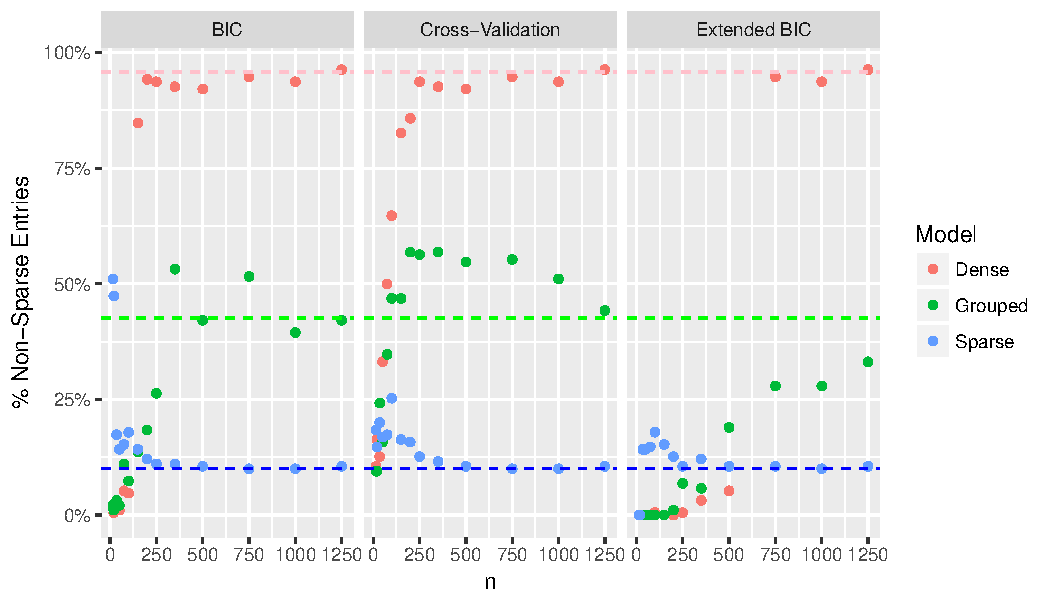
\includegraphics[scale=0.4]{Sparsity} }

}

\label{fig:example}
\end{figure}

\noindent The cross-validation and BIC penalty parameter selection
methods performed similarly in the limit $n\rightarrow\infty$. The
BIC criteria perform better for the sparse model but poorly on the
dense model (especially extended BIC) for small $n$. The BIC penalty
appears to generally induce greater sparsity in the resulting estimated
precision matrix than the CV approach at the same $n$. 

\noindent In practice, this suggests that the BIC approach may be
advantageous when the researcher expects a highly sparse $\Theta$,
whereas the CV approach may be preferred when $\Theta$ is dense or
not known to be sparse. In the appendix we show the true sparse, grouped,
and dense graphs and the estimated graphs for $n=15$, $n=150$, and
$n=1250$ under $\lambda_{CV}$, $\lambda_{BIC}$, and $\lambda_{Ext.BIC}$.
\end{singlespace}
\begin{singlespace}

\section{Data Analysis Application: Malaria Gene Pathway}
\end{singlespace}

\begin{singlespace}
\noindent Due to the high cost of the technologies, the sample size
is always much smaller than the number of genes, rendering the gene
covariance matrix noninvertible, and hence makes it impossible to
obtain the precision matrix that indicates the conditional dependence
among the genes. On the other hand, the pathways (i.e. dependence
between genes) are sparse among genes, therefore graphical LASSO provides
an effective way of estimation such a dependency relation between
genes represented by the vertexes and the dependency represented by
the edges.

\noindent Gene Expression Omnibus (GEO) is a public database that
provides gene expression data with easy user access. Among the 4,349
datasets available in this database, we found gene expression data
in malaria infection (GSE 5418) that provides pairwise transcription
readings (experimental malaria-infected versus baseline uninfected)
for 22 human subjects. The expression data for the 22 individuals
were generated from Affymetrix's GPL96 microarray platform. Note that
the cost of microarray technology has decreased significantly over
the years (and is much lower than that of the next sequencing technologies),
but the total expense of the biological analysis can still be high
when the number of test subjects is large. GSE 5418 is the largest
dataset we can find on GEO that has pairwise design on human subjects,
and it provides readings on 22,283 different genes and genomic segments.

\noindent To identify the differentially expressed genes, we utilize
the DIME software \cite{DIME} (Differential Identification using
Mixture Ensemble) that considers gene log ratios following some finite
mixture model. The models under evaluation are gamma-normal-gamma
(gng), normal-uniform (nudge), and multiple normal-uniform (inudge).
Since the log intensities also play a role in indicating genetic signal™
significance, the DIME software applies Huber weights that upweight
genes with larger log Gaussian intensities. Here, we have tens of
thousands of genes, so the false discovery rate (FDR) is used for
multiple comparison correction.

\noindent The interaction among these differentially expressed genes
are of particular interest. However, the number of differentially
expressed genes may still be larger than the sample size and the covariance
matrix is still noninvertible. Hence, graphical LASSO can be applied
so that precision matrix can be achieved and weak conditional dependence
among genes will be penalized to 0. Of course, we can use cross validation
or extended BIC to identify the ideal tuning parameter for the restriction.
Nevertheless, the graph resulting from the precision matrix should
be sparse enough to only show the important information, so the number
of connections can be prefixed as well.

\noindent We provide the results of applying graphical LASSO to our
data under two scenarios. In the first, we focus on the genes that
belong to the interferon signaling pathways, while, in the second
we expand our focus to the top 100 differentially expressed genes
(that have FDR smaller than $10^{-7}$). In both cases the penalty
parameter was chosen under the extended BIC criterion. Our estimated
graphs are both shown on the following page.

\noindent The genes that extend multiple connections are called the
hub genes and they can be considered as the control center for the
infection process, as they share conditional dependence with various
other genes. The hub genes are essential for diagnosing and treating
diseases, and they are the keys for the genetic medicine development.
In the plots that follow, CCL2 is a hub gene with several connections,
and it is an immunoregulatory gene from the Chemokine family. The
hub gene, CCL2, is apparent in both of the estimated graphs below
Figure \ref{fig:No-Pathway-(Top}.

\noindent 
\begin{figure}
{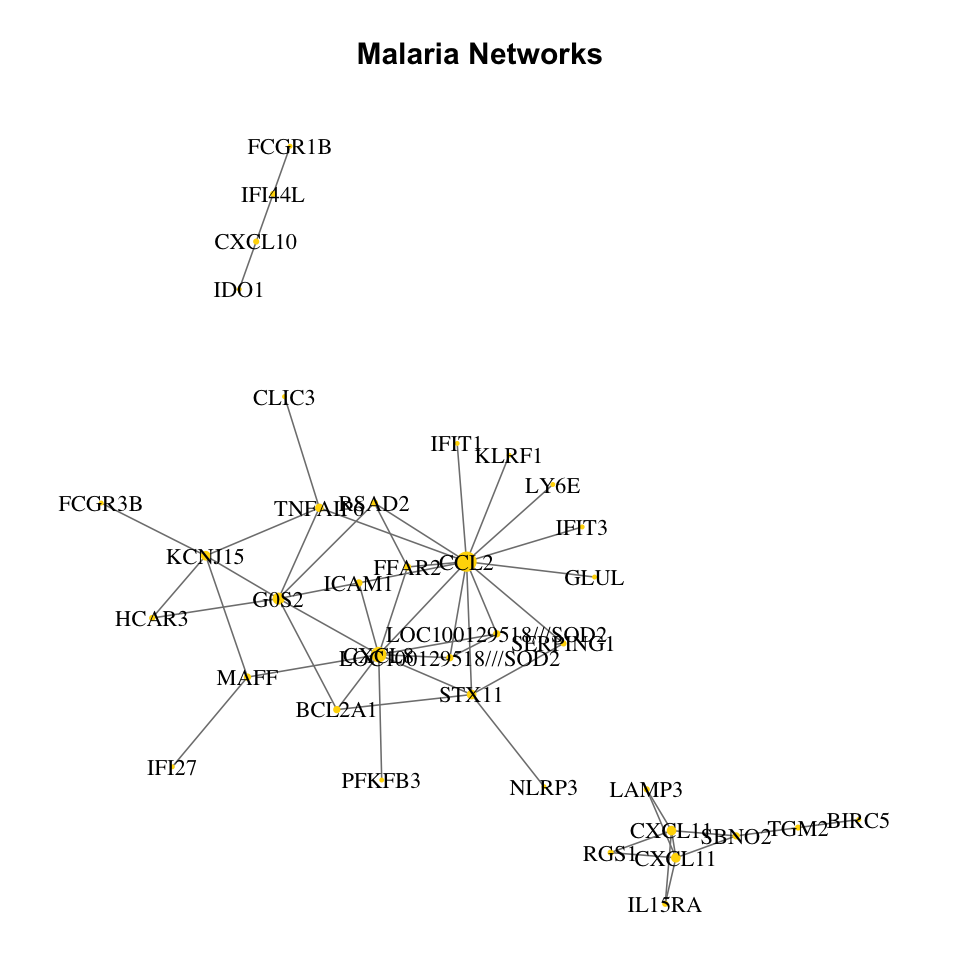
\includegraphics[scale=0.2]{NoPathway} }

\caption{\label{fig:No-Pathway-(Top}No Pathway (Top 100) Estimate}
\end{figure}

\end{singlespace}
\begin{singlespace}

\section{Conclusion}
\end{singlespace}

\begin{singlespace}
\noindent As we have seen, graphical LASSO \cite{FHT2008} offers
an efficient, quick solution to the problem of estimating the precision
matrix of an undirected graph model. It applies very well to the data
set where there exists some kind of sparsity. Compared to the naive
approach of inverting the empirical covariance matrix, graphical LASSO
provides a more consistent estimate to the precision matrix $\Theta$
with sparsity constraints such as high dimensionality. Moreover, numerically
graphical LASSO is more stable compared to inversion of covariance.
In the second perspective, we can equivalently treat the graphical
LASSO as conditional iterative least square estimation, which provides
more insights into the dependency relations between the random variables
represented by the vertexes. This makes the result of the method very
intepretable especially attractive in fields such as high dimensional
network, spatial analysis and genetics.

\noindent In addition, we discussed three ways proposed in the literature
for selection of an optimal tuning parameter $\lambda$. Methods of
cross-validation, BIC and extended BIC each have their strengths and
weaknesses which we investigated deeply in our simulation study. Although
the problem of choosing a penalty parameters for a regularization
method like graphical LASSO is generally difficult \cite{foygel,GAO},
we still implement and evaluate three different ways of choosing penalty
parameters therein. To sum up our result, BIC or information criteria
approach may be advantageous when the researcher expects a highly
sparse precision matrix $\Theta$, whereas the cross-validation approach
may be preferred when $\Theta$ is dense or not known to be sparse.

\noindent Graphical LASSO is a valuable tool in network construction
when sparsity is the goal or when the number of variables $p$ is
larger than the sample size $n$ as we discussed above \cite{DIME}.
We illustrated this point further in our gene analysis example, where
the pathway dependency between genes are sparse due to the sequencing
technologies. In the real data application, we utilize the malaria
data from 22 subjects on more than 20,000 genes. Even though the number
of genes is significantly reduced from DE gene selection, it is still
much higher than the number of subjects. By applying graphical LASSO,
we are able to penalize the weak connections and construct a precision
matrix to indicate conditional dependence.

\noindent In all, we explained the methodology of the graphical LASSO
in two equivalent ways of precision matrix based undirected graph
\cite{FHT2008} and the iterative least square estimation \cite{Meinshausen=00003D000026B=00003D0000FChlmann2006};
and then discussed the effect of penalty parameters by simulation
study comparing existing criteria \cite{foygel,GAO} and eventually
we apply the graphical LASSO methodology onto the genetic analysis
and showed its effectiveness when the dependency between variables
are sparse \cite{DIME}.

\noindent \newpage{}
\end{singlespace}
\begin{thebibliography}{1}
\begin{singlespace}
\bibitem{FHT2008}Friedman, Jerome, Trevor Hastie, and Robert Tibshirani.
\textquotedbl{}Sparse inverse covariance estimation with the graphical
LASSO.\textquotedbl{} Biostatistics 9.3 (2008): 432-441.

\bibitem{FHT2001}Friedman, Jerome, Trevor Hastie, and Robert Tibshirani.
The elements of statistical learning. Vol. 1. New York: Springer series
in statistics, 2001.

\bibitem{foygel} Foygel, R., \& Drton, M. \textquotedbl{}Extended
Bayesian information criteria for Gaussian graphical models.\textquotedbl{}
In Advances in Neural Information Processing Systems 23: 24th Annual
Conference on Neural Information Processing Systems 2010, NIPS 2010.

\bibitem{GAO}Gao, Xin, Daniel Pu, Yuehua Wu, and Hong Xu. \textquotedbl{}Tuning
parameter selection for penalized likelihood estimation of Gaussian
graphical model.\textquotedbl{} Statistica Sinica 22 (2012): 1123-1146.

\bibitem{Meinshausen=00003D000026B=00003D0000FChlmann2006}Meinshausen,
Nicolai, and Peter . \textquotedbl{}High-dimensional graphs and variable
selection with the LASSO.\textquotedbl{} The annals of statistics
(2006): 1436-1462.

\bibitem{Mazumder2012}Mazumder, Rahul, and Trevor Hastie. \textquotedbl{}The
graphical LASSO: New insights and alternatives.\textquotedbl{} Electronic
journal of statistics 6 (2012): 2125.

\bibitem{DIME}Taslim, Cenny, Tim Huang, and Shili Lin. \textquotedbl{}DIME:
R-package for identifying differential ChIP-seq based on an ensemble
of mixture models.\textquotedbl{} Bioinformatics 27.11 (2011): 1569-1570.

\bibitem{Wright2015}Wright, Stephen J. \textquotedbl{}Coordinate
descent algorithms.\textquotedbl{} Mathematical Programming 151.1
(2015): 3-34. 
\end{singlespace}
\end{thebibliography}

\end{document}
